\documentclass{article}
\usepackage[utf8]{inputenc}
\usepackage{graphicx}
\title{Problem 1 (b) Context of Use Model}
\author{Arnab Roy, Saraswati Saud, Shagun Sharma, Pavit Srivatsan }

\begin{document}
\date{}
\maketitle

\section{Introduction}
Definition [Context of Use]. A description of the conditions under which a softwaresystem will be used in a normal working situation.
\section{Context Diagram}
\begin{figure}[htp]
    \centering
    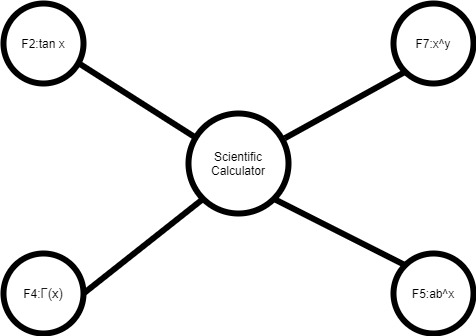
\includegraphics[width=10cm]{ContextDiagram}
    \caption{Context Diagram for Scientific Calculator}
    \label{fig:context_diag}
\end{figure}
A context diagram is a diagram represents a context of use model pictorially [Girvan,
Paul, 2017, Chapter 11; Laplante, 2018, Chapter 3; Aschauer, Hruschka, Lauenroth,
Meuten, Rogers, 2018, Section 2.1.5.1].
\\The scientific calculator constructed for the project submission encompasses the mathematical funtions $tan(x)$, $\Gamma(x)$, $ab^x$, $x^y$ as shown in the Figure 1.
\section{Context of Use Model}
\begin{figure}[htp]
    \centering
    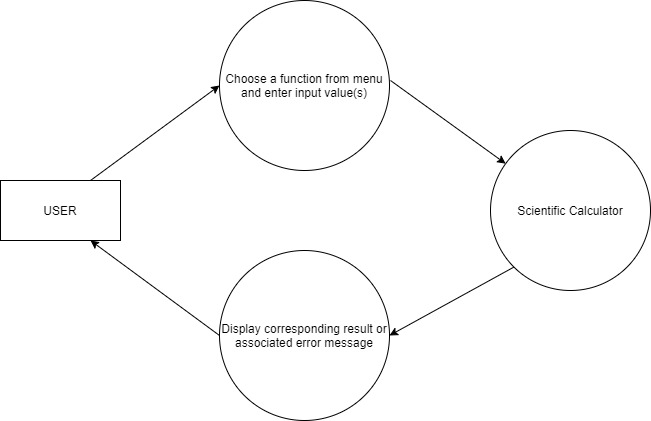
\includegraphics[width=10cm]{contextofuse}
    \caption{Context of Use Model for Scientific Calculator}
    \label{fig:context_diag}
\end{figure}
The context of use model is shown in the figure. 
\subsection{Users}
\textbf{Developers:}\\
The developers of the system use it frequently to check if the system is working as expected.\\\\
\textbf{Testers:}\\
The testers of the system test the functions are working correctly.\\\\
\textbf{Assessing Team:}\\
The assessor team will need to assess the project implementation.\\\\
\textbf{Students and Peers:}\\
Students and peers of the course may use the calculator to find the results of the above-specified function. It can serve as a future reference for implementing a scientific calculator.\\\\
\textbf{Researchers and Other Academicians:}\\
Researchers and other academicians can be interested in the system to calculate the result of the function. Identify differences in implementation, the behaviour of the system to compare and contrast.
\begin{thebibliography}{9}
\bibitem{Context of use}
Understanding Context,\\
\url{https://users.encs.concordia.ca/~kamthan/courses/soen-6011/understanding_context.pdf}
\end{thebibliography}
\end{document}

